\documentclass{article}
\usepackage{amsfonts, amsmath, amssymb, amsthm, dsfont} % Math notations imported
\usepackage{enumitem}
\usepackage{graphicx}
\usepackage{setspace}
\usepackage{indentfirst}
\usepackage[margin=1in]{geometry}
\graphicspath{{./images/}} % Path to images

% \begin{figure}[htb!]
%      \centering
%      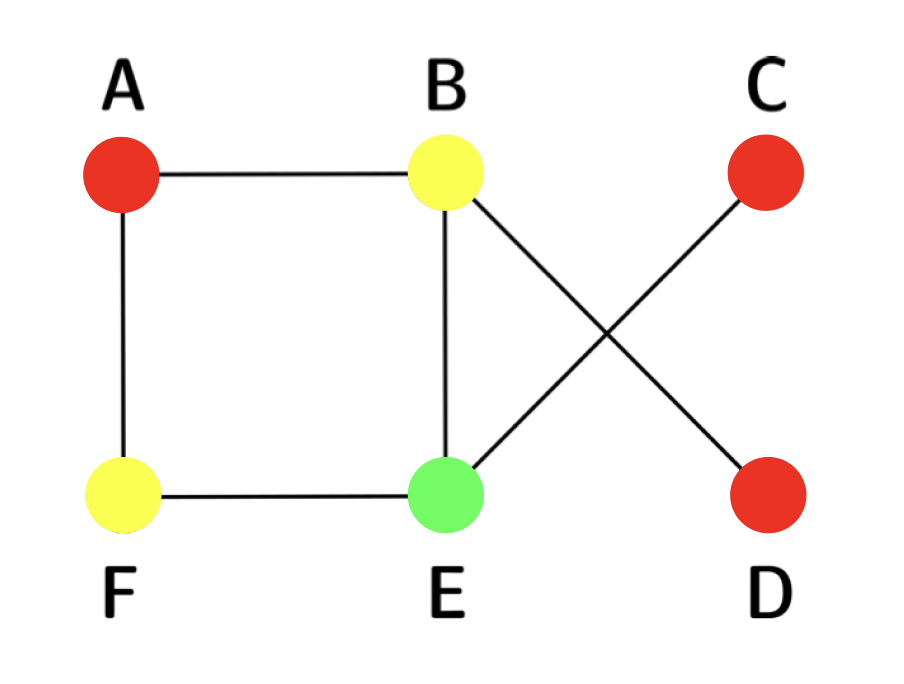
\includegraphics[scale=0.5]{coloring.png}
%      \caption{Coloring of the graph.}
% \end{figure}

% \begin{figure}[htb]
%     \qquad
%     \begin{minipage}{.4\textwidth}
%         \centering
%         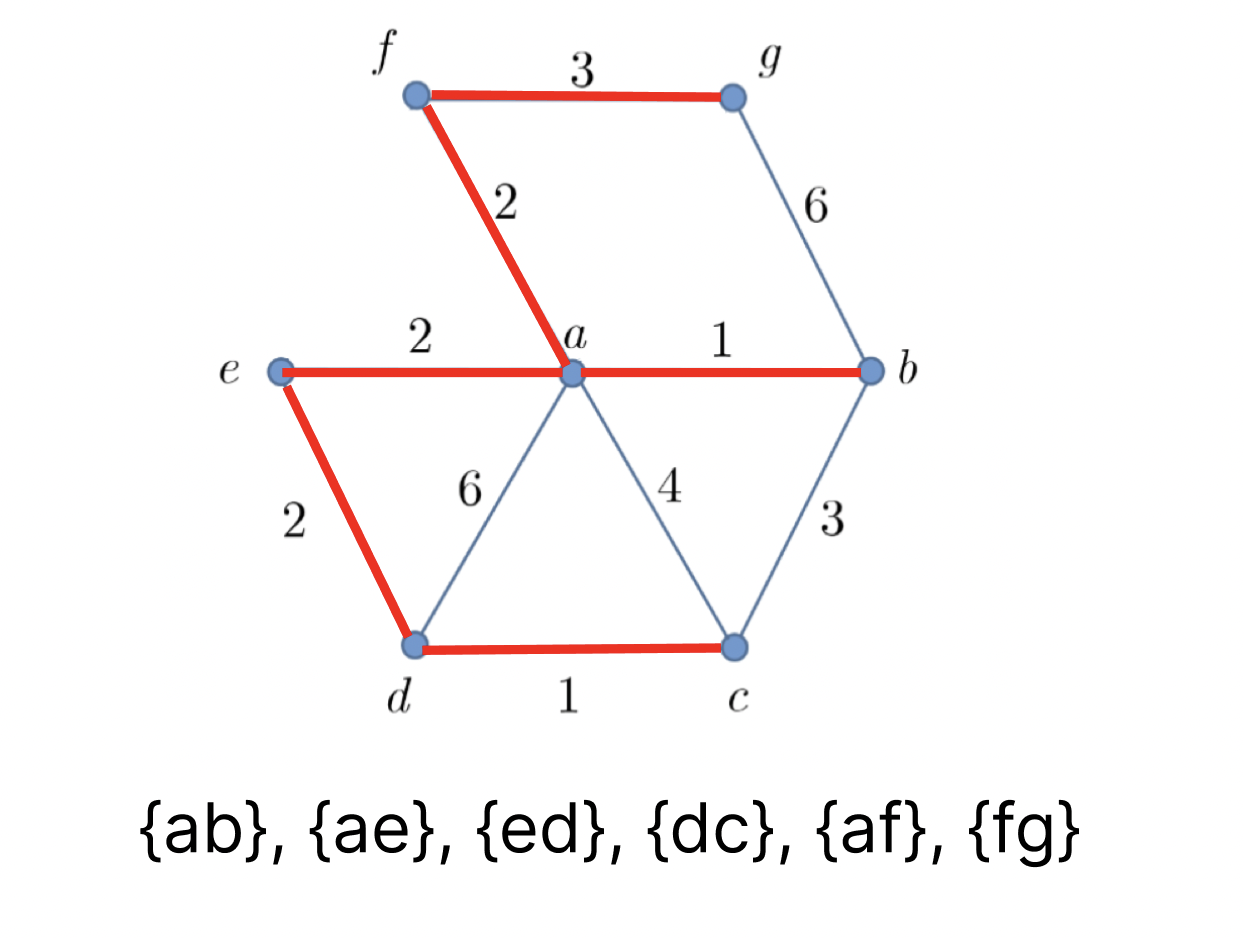
\includegraphics[scale=0.35]{prims.png}
%         \caption{}
%     \end{minipage}    
%     \qquad
%     \begin{minipage}{.4\textwidth}
%         \centering
%         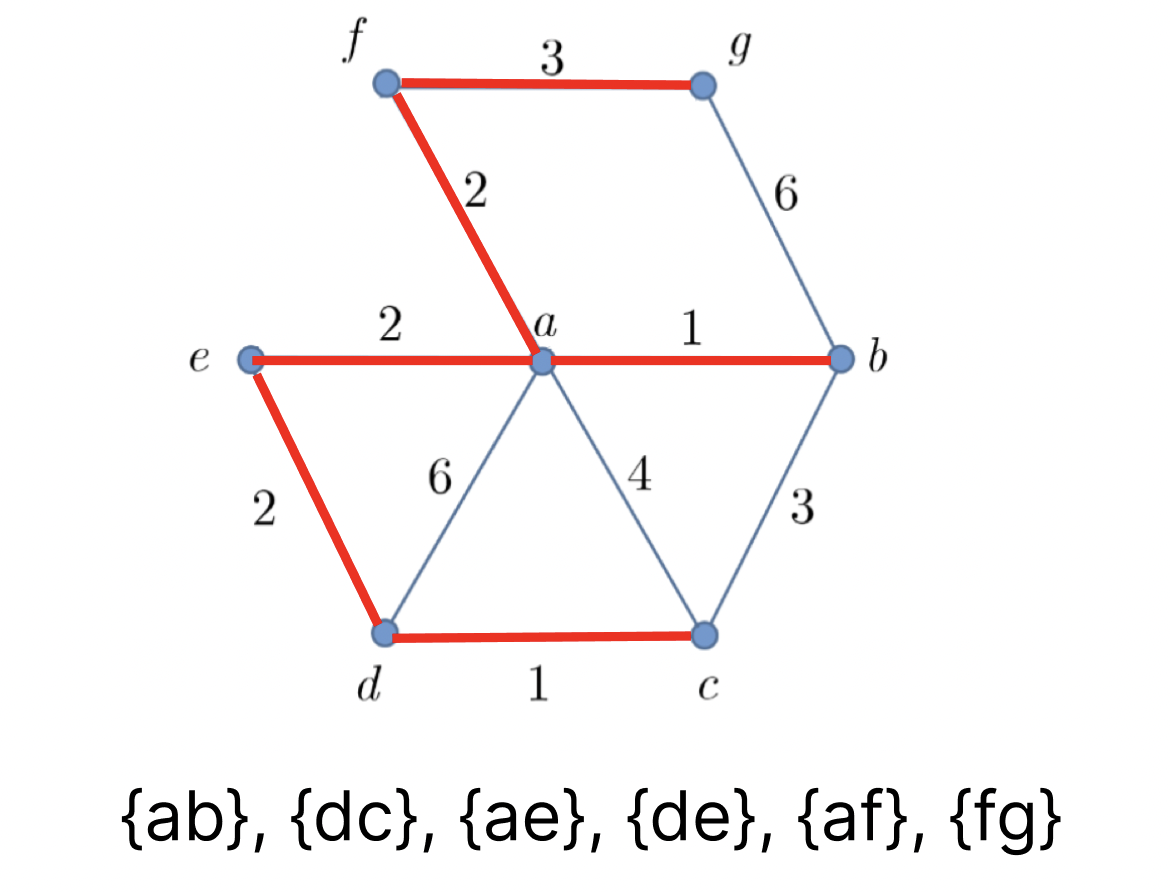
\includegraphics[scale=0.35]{kruskal.png}
%         \caption{}
%     \end{minipage}        
% \end{figure} 

\newtheorem{thm}{Theorem}
\newtheorem{proposition}[thm]{Proposition}
\newtheorem{corollary}[thm]{Corollary}
\newtheorem{lemma}[thm]{Lemma}

\newcommand*{\Var}{\ensuremath{\mathrm{Var}}}
\newcommand*{\Cov}{\ensuremath{\mathrm{Cov}}}
\newcommand*{\Corr}{\ensuremath{\mathrm{Corr}}}
\newcommand*{\Bias}{\ensuremath{\mathrm{Bias}}}
\newcommand*{\MSE}{\ensuremath{\mathrm{MSE}}}
\newcommand*{\range}{\ensuremath{\mathrm{range}}\,}
\newcommand*{\spann}{\ensuremath{\mathrm{span}}\,}
\newcommand*{\nul}{\ensuremath{\mathrm{null}}\,}
\newcommand*{\dom}{\ensuremath{\mathrm{dom}}\,}
\renewcommand*{\implies}{\ensuremath{\Longrightarrow}}
\renewcommand*{\impliedby}{\ensuremath{\Longleftarrow}}
\newcommand*{\Z}{\ensuremath{\mathbb{Z}}}
\newcommand*{\Q}{\ensuremath{\mathbb{Q}}}
\newcommand*{\R}{\ensuremath{\mathbb{R}}}
\newcommand*{\F}{\ensuremath{\mathbb{F}}}
\newcommand*{\C}{\ensuremath{\mathbb{C}}}
\newcommand*{\N}{\ensuremath{\mathbb{N}}}
\newcommand*{\E}{\ensuremath{\mathds{E}}}
\renewcommand*{\P}{\ensuremath{\mathds{P}}}
\newcommand*{\p}{\ensuremath{\mathcal{P}}}

% title information
\title{Math 110 HW12}
\author{Neo Lee}
\date{11/25/2023}

\setstretch{1.15}
% main content
\begin{document} 

% placing title information; comment out if using fancyhdr
\maketitle 

\subsection*{Problem 1.}
Let $T\in {\cal L} (V,W)$. Prove
\begin{description}
\item{(a)} $T$ is injective if and only if $T^*$ is surjective;
\item{(b)} $T^*$ is injective if and only if $T$ is surjective.
\end{description}
\begin{proof}\indent
    \begin{enumerate}[label=(\alph*)]
        \item
        \begin{align*}
            \nul T = \{0\} & \iff (\range T^*)^\perp = \{0\} \\
            & \iff \range T^* = V.
        \end{align*}

        \item
        \begin{align*}
            \nul T^* = \{0\} & \iff (\range T)^\perp = \{0\} \\
            & \iff \range T = W.
        \end{align*}
    \end{enumerate}
\end{proof}

\newpage
\subsection*{Problem 2.}
Suppose $S$, $T \in {\cal L}(V)$ are self-adjoint.  Prove that $ST$ is self-adjoint if and only if $ST=TS$.
\begin{proof}
    We will prove both direction in one go. Let $v, w\in V$,
    \begin{align}
        ST = TS & \iff \overline{\langle w, STv\rangle} = \overline{\langle w, TSv\rangle} \\
        & \iff \langle STv, w\rangle = \langle TSv, w\rangle \\
        & \iff \langle v, (ST)^*w \rangle = \langle Sv, T^*w\rangle \\
        & \iff \langle v, (ST)^*w \rangle = \langle v, S^*T^*w\rangle \\
        & \iff \langle v, (ST)^*w\rangle = \langle v, STw\rangle \\
        & \iff (ST)^* = ST.
    \end{align}
    (1) is by the uniqueness of complex conjugate and the Riesz representation theorem. 
    (6) is by the uniqueness of the Riesz representation theorem.
\end{proof}

\newpage
\subsection*{Problem 3.}
Let $P\in {\cal L}(V)$  be such that $P^2=P$. Prove that there is a subspace $U$ of $V$ such that $P_U=P$ if and only if $P$ is self-adjoint.
\begin{proof}
    \textbf{Forward direction:} Let $W = \nul P$, then $U\oplus W = V$ because $P$ is an orthogonal 
    projection.

    Now, let $x, y\in V$, 
    \begin{align*}
        \langle x, P^*y\rangle = \langle Px, y\rangle & = \langle P(x_u + x_w), y_u + y_w \rangle \\
        & = \langle x_w, y_u+y_w\rangle \\
        & = \langle x_u, y_u \rangle + \langle x_u, y_w \rangle \\
        & = \langle x_u, y_u \rangle \\
        & = \langle x_u + x_w, y_u \rangle \\
        & = \langle x, Py\rangle.
    \end{align*}
    Hence, by the uniqueness of the Riesz representation theorem, $P^* = P$.

    \textbf{Backward direction:} $P$ is self-adjoint and hence normal. Then by either the complex 
    or the real spectral theorem, $V$ can be decomposed into a direct sum of eigenspaces of $P$ 
    where all the eigenvectors are orthonormal. Since $P$ is self-adjoint, all its eigenvalues are 
    real. Also, $P^2 = P$ means the only eigenvalues can only be $0$ or $1$. Now, let $U$ be the 
    eiganespace of $P$ with eigenvalue $1$ and $W$ be the eigenspace of $P$ with eigenvalue $0$. 
    We know $U\perp W$ since $P$ has orthonormal eigenvectors.
    Then for any $v\in V$, 
    $$Pv = P(\underbrace{u + w}_{u\in U, w\in W}) = u.$$ Hence, by definition of orthogonal
    projection, $P_U = P$.
\end{proof}

\newpage
\subsection*{Problem 4.}
Let $n\in \N$ be fixed. Consider the real space 
$V := \spann (1, \cos x, \sin x, \cos 2x, \sin 2x, \ldots, \cos nx, \sin nx)$
with inner product $$\langle f, g\rangle := \int_{-\pi}^\pi f(x) {g(x)} dx . $$ 
Show that the differentiation operator $D \in {\cal L}(V)$ is {\it anti-Hermitian}, i.e., satisfies $D^*=-D$. 
\begin{proof}
    Let $f, g\in V$, then
    \begin{align*}
        \langle Df, g\rangle & = \int_{-\pi}^\pi Df(x) g(x) dx \\
        & = \int_{-\pi}^\pi f'(x) g(x) dx \\
        & = \left. f(x)g(x) \right|_{-\pi}^\pi - \int_{-\pi}^\pi f(x) g'(x) dx \\
        & = -\int_{-\pi}^\pi f(x) g'(x) dx \\
        & = -\langle f, Dg\rangle.
    \end{align*}
    Hence, by the uniqueness of the Riesz representation theorem, $D^* = -D$.

    $$\left. f(x)g(x) \right|_{-\pi}^\pi = 0$$ is true because $f$ and $g$ can be written as 
    $$\alpha + \sum_{k=1}^{n}a_k\sin (kx) + b_k\cos (kx)$$
    but with different coefficients. Either way, $f(\pi) = f(-\pi)$ and $g(\pi)=g(-\pi)$ because 
    all the $\sin$ functions evaluated at $\pi, -\pi$ are 0 and all the $\cos$ functions are even 
    functions. Therefore, $$f(\pi)g(\pi) = f(-\pi)g(-\pi) \iff f(\pi)g(\pi) - f(-\pi)g(-\pi) = 0.$$
\end{proof}

\newpage
\subsection*{Problem 5.}
Suppose $T$ is normal. Prove that, for any $\lambda \in \F$ and any $k\in \N$,
$$ {\rm null}\, (T-\lambda I)^k = {\rm null}\, (T-\lambda I).$$
\textbf{Lemma:} Let $S$ be a self-adjoint operator, then for any $k\in \N$,
$${\rm null}\, S^k = {\rm null}\, S.$$
\begin{proof}[\textbf{Proof of Lemma}]
    Assume this is not true, then we take the minimal counterexample. Let $n \ge 2$ be the minimal
    counterexample.

    Clearly, $\nul S\subseteq \nul S^n$. Let $v\in \nul S^n$, then 
    \begin{align*}
        \langle S^nv, S^{n-2}v\rangle = 0 & \iff \langle S^{n-1}v, S^{n-1}v\rangle = 0 \\
        & \iff \|S^{n-1}v\|^2 = 0 \\
        & \iff S^{n-1}v = 0 \\ 
        & \iff v\in \nul S^{n-1} \\
        & \iff v\in \nul S \qquad (\because S^n \text{ is the minimal counterexample}),
    \end{align*}
    which is a contradiction to the minimality of $n$. Hence, $\nul S^k = \nul S$.
\end{proof}
\begin{proof}[\textbf{Proof of Problem 5}]
    Clearly, $\nul (T-\lambda I)\subseteq \nul (T-\lambda I)^k$. Let $v\in \nul (T-\lambda I)^k$, 
    then let 
    $$S = (T-\lambda I)^*(T-\lambda I),$$
    where $S$ is self-adjoint because 
    $$S^* = [(T-\lambda I)^*(T-\lambda I)]^* = (T-\lambda I)^*(T-\lambda I) = S.$$
    Also, 
    \begin{align*}
        S^k & = (T-\lambda I)^*(T-\lambda I) \cdots (T-\lambda I)^*(T-\lambda I)\\
        & = \left[(T-\lambda I)^*\right]^k(T-\lambda I)^k,
    \end{align*}
    by repeatedly swapping the positions of $(T-\lambda I)^*$ and $(T-\lambda I)$
    because $(T-\lambda I)$ is normal.
    Now, let $v$ in $\nul (T-\lambda I)^k$, clearly $v\in \nul S^k$. Then by the lemma,
    $v\in\nul S$. Hence, 
    \begin{align*}
        \langle (T-\lambda I)^*(T-\lambda I)v, v\rangle = 0 & \iff \langle (T-\lambda I)v, (T-\lambda I)v\rangle = 0 \\
        & \iff \|(T-\lambda I)v\|^2 = 0 \\
        & \iff (T-\lambda I)v = 0 \\
        & \iff v\in \nul (T-\lambda I).
    \end{align*}
    Thus we proved the inclusion of $\nul (T-\lambda I)^k \subseteq \nul (T-\lambda I)$.
\end{proof}

\end{document}
